% ===========================================================================
% Supplement to: PakEmis v1.0: an evidence-graded public-data reconstruction of
% Pakistan's non-LULUCF greenhouse-gas emissions, FY2015-16 to FY2023-24
%
% A separate document (article class, single-column A4) for the reasons the main
% article states: the air-pollutant layer is a companion product of markedly lower and
% MORE UNEVEN assurance than the greenhouse-gas dataset, and a ranking drawn across it is
% easy to over-read; the parallel-table rule and the reproduction detail are method
% record rather than data description; and the claim matrix is a table too long for the
% article. Wide tables fit here without becoming table* floats.
%
% Sections: S1 the air beta - S2 key categories (pointer: the analysis is in the main
% article) - S3 the parallel-table rule (05_factor_tables) - S4 reproduction, months,
% geography and sources (14_appendix) - S5 the claim matrix (generated/claim_matrix.tex,
% written by scripts/make_claim_matrix.py).
%
% Build: latexmk -pdf supplement.tex   (the Makefile does this automatically, after the
% main article and before its second pass, because the two documents resolve each
% other's labels through xr until the prose pass replaces those \ref with pointers)
% ===========================================================================
\documentclass[a4paper,11pt]{article}
\usepackage[margin=0.85in]{geometry}
% ===========================================================================
% Shared preamble for every manuscript in this repository.
%
% Papers using it:
%   paper/            agriculture inventory
%   paper_nowcast/    agricultural nowcasting
%   paper_national/   the nine-sector national inventory
%   notes/<sector>/   one data note per non-agriculture sector
%
% It exists because paper/ and paper_nowcast/ began as copies of one another
% and had already drifted five lines apart before a third manuscript existed.
% Eleven copies would drift eleven ways, and a macro that renders differently
% in two papers is the kind of defect nobody notices until proof stage.
%
% \graphicspath is deliberately NOT set here - each manuscript sets its own
% after \input{...preamble}, because figures live beside the document.
% ===========================================================================

\usepackage[utf8]{inputenc}
\usepackage[T1]{fontenc}
\usepackage{amsmath,amssymb}
\usepackage{graphicx}
\usepackage{booktabs}
\usepackage{multirow}
\usepackage{siunitx}
\usepackage[colorlinks=true,citecolor=blue,linkcolor=blue,urlcolor=blue]{hyperref}
% Document-information metadata for every PDF in the bundle (the seventh review noted
% the shipped PDFs carried none). Documents that set their own \hypersetup{pdftitle=...}
% keep it - hyperref takes the LAST setting, and this shared block runs first. Full
% tagged-PDF (tagpdf / \DocumentMetadata) is deliberately not attempted here: the
% installed LaTeX toolchain's support is not uniform across sixteen documents, and a
% half-tagged bundle is worse than an honestly untagged one; deferred deliberately.
\hypersetup{
  pdfauthor={Rehan Ahmad, Pakistan Air Quality Initiative (PAQI)},
  pdfsubject={A reproducible ten-sector national greenhouse-gas inventory
              for Pakistan},
  pdfkeywords={Pakistan, greenhouse gas inventory, IPCC 2006 Guidelines, MRV,
               reproducible research, emissions, air pollutants},
}
\usepackage{caption}
\captionsetup[table]{position=below}
\usepackage{enumitem}
\usepackage{xcolor}
\usepackage{float}
\usepackage{placeins}
\usepackage{tabularx}
\usepackage{natbib}
\usepackage{tikz}
\usetikzlibrary{arrows.meta,positioning,fit,backgrounds}

\setlength{\emergencystretch}{3em}

% Looser float placement to prevent pile-up in two-column mode.
\renewcommand{\topfraction}{0.95}
\renewcommand{\bottomfraction}{0.85}
\renewcommand{\textfraction}{0.05}
\renewcommand{\floatpagefraction}{0.85}
\setcounter{topnumber}{4}
\setcounter{bottomnumber}{3}
\setcounter{totalnumber}{6}

% ---------------------------------------------------------------------------
% Custom shorthand: in macros.tex since the ESSD re-targeting, because the national
% article compiles under the Copernicus class and cannot take this preamble (the class
% loads its own packages) but needs exactly the same macros. This file inputs it so that
% every other manuscript keeps compiling unchanged.
%
% THREE relative paths, because \input resolves against the COMPILE DIRECTORY and not
% against this file, so the depth is a property of whoever is building:
%   ../paper_common      a manuscript compiled from one level down
%   ../../paper_common   papers/<sector>/ and notes/<sector>/
%   ../../../paper_common  paper_national/versions/<v>/, since the national paper was
%                          versioned - that move is what added this third arm, and the
%                          supplement failed with "../../paper_common/macros.tex not
%                          found" until it was here
% A fourth depth needs a fourth arm, which is the cost of keeping a bare `latexmk` in a
% manuscript directory working without a TEXINPUTS set for it.
% ---------------------------------------------------------------------------
\IfFileExists{../paper_common/macros.tex}%
  {\input{../paper_common/macros}}%
  {\IfFileExists{../../paper_common/macros.tex}%
    {\input{../../paper_common/macros}}%
    {% ===========================================================================
% paper_common/macros.tex - the shorthand every manuscript shares.
%
% Split from preamble.tex in the ESSD re-targeting: the national article now compiles
% under the Copernicus class, which loads its own packages and forbids most of what
% preamble.tex sets (geometry-like options, a second hyperref, placeins), but it needs
% exactly the same shorthand as the sector reports. The macros therefore live here, on
% their own, and preamble.tex inputs this file so that every other manuscript keeps
% compiling unchanged. A macro that renders differently in two documents is the defect
% this file exists to prevent; define it once.
%
% Requires: siunitx (for \DeclareSIUnit and \si) - the caller loads it.
% ===========================================================================

% Gas and pollutant names.
\newcommand{\COtwo}{CO\textsubscript{2}}
\newcommand{\COe}{CO\textsubscript{2}e}
\newcommand{\CHfour}{CH\textsubscript{4}}
\newcommand{\NtwoO}{N\textsubscript{2}O}
\newcommand{\NHthree}{NH\textsubscript{3}}
\newcommand{\NOx}{NO\textsubscript{x}}
\newcommand{\SOtwo}{SO\textsubscript{2}}
\newcommand{\PM}{PM\textsubscript{2.5}}
\newcommand{\MCF}{MCF}
\newcommand{\Mt}{\text{Mt~\COe}}
\newcommand{\tCha}{\si{\tonne\per\hectare}}
\newcommand{\AFOLU}{AFOLU}
\newcommand{\GLW}{GLW\,4}
\newcommand{\EFone}{EF\textsubscript{1}}

% siunitx: allow Mt, Tg, ha, head, yr, dB
\DeclareSIUnit{\head}{head}
\DeclareSIUnit{\yr}{yr}
\DeclareSIUnit{\dB}{dB}

% A file name is the one long unbreakable token these documents are full of -
% \texttt{waste\_air\_pollutants\_2024.csv} is wider than a two-column measure and TeX prints
% it past the margin rather than breaking it. Allowing a break AFTER each escaped underscore
% costs nothing and inserts no hyphen, which matters: a hyphenated file name is a wrong file
% name. This is one line because every such name in every document is written with \_.
\let\pkinvunderscore\_
\renewcommand{\_}{\pkinvunderscore\allowbreak}
}}
% Long unbreakable strings - output filenames, module paths, URLs in \texttt - do not fit a
% two-column measure and TeX prints them past the margin rather than breaking them. Nothing
% read the log, so 47 of those overruns shipped across seven documents. Emergency stretch lets
% the paragraph loosen instead, and \texttt is taught to break at the punctuation these names
% actually contain.
\emergencystretch=6em


\hypersetup{pdftitle={Supplement to PakEmis v1.0},
            pdfauthor={Rehan Ahmad}}
\usepackage{xr}
\externaldocument[][nocite]{paper_national}   % nocite: labels only, not the article's \bibcite
\graphicspath{{../../figures/}}

\sloppy
\emergencystretch=2em
% The parallel-table rule's five-column table (05_factor_tables) was laid out for a
% full-width two-column float; at this text width its column padding overran by half a
% point. One point less padding per column side fits it with margin to spare.
\setlength{\tabcolsep}{5pt}

\renewcommand{\thesection}{S\arabic{section}}
\renewcommand{\thetable}{S\arabic{table}}
\renewcommand{\thefigure}{S\arabic{figure}}

% The moved appendix keeps its four \section lines; under one supplement section they
% become subsections (the same device the main article's containers use).
\newcommand{\pkinvDemoteFragment}{\begingroup
  \let\section\subsection
  \let\subsection\subsubsection}
\newcommand{\pkinvEndFragment}{\endgroup}

\title{Supplement to: PakEmis v1.0: an evidence-graded public-data reconstruction of
Pakistan's non-LULUCF greenhouse-gas emissions, FY2015--16 to FY2023--24\\[6pt]
\large The air beta, the parallel-table rule, the reproduction record and the claim matrix}
\author{Rehan Ahmad\\ \small Pakistan Air Quality Initiative (PAQI), Karachi, Pakistan}
\date{}

\begin{document}
\maketitle

%% GENERATED by scripts/make_release_cover.py from outputs/release_manifest.json.
%% Do not edit: the edit will be overwritten and CI diffs the result.
\newcommand{\ReleaseCover}{%
\begin{center}\small
\setlength{\fboxsep}{4pt}%
\fbox{\begin{minipage}{\dimexpr\linewidth-2\fboxsep-2\fboxrule\relax}\footnotesize
\textbf{Release provenance.} This document describes PakEmis under the period, configuration and source boundaries specified in its methods. The identifiers below link it to the accompanying products and source register.\\[2pt]
\begin{tabular}{@{}p{0.32\linewidth}@{\hspace{0.03\linewidth}}p{0.65\linewidth}@{}}
Release version & \texttt{1.0.0rc69} \\
Commit & \texttt{d8d874622f9a} \\
Reporting period & July 2015--June 2025 (ten fiscal years) (2015-07-01 to 2025-06-30) \\
Reference & S\_TAN (household survey; TAN nitrogen) \\
FY2023--24 total & 444.61 Mt \COe{} (AR5) under S\_TAN, the reference; 449.85 Mt under L\_TAN \\
Release manifest & \texttt{ac0ffe93ad9fcd88} (SHA-256 of \texttt{outputs/release\_manifest.json}, first 16) \\
Source manifest & \texttt{c1be6d314cfce1ea} (SHA-256 of \texttt{data/manifests/source\_manifest.csv}, first 16) \\
Data-description article & \texttt{paper\_national/} (ESSD, in preparation), same release
\end{tabular}
\end{minipage}}
\end{center}}

\ReleaseCover

This supplement carries what a reader of the main article may need and the article itself
does not hold: the air-pollutant beta layer (Section~\ref{sec:airbeta}), which is
deliberately kept out of the greenhouse-gas result; a pointer to the key-category
analysis (Section~\ref{sup:keycat}); the parallel-table rule in the IPCC defaults
(Section~\ref{sec:factors}); the reproduction record, with where the months and the
geography come from and the source-by-source account (Section~\ref{sup:reproduction});
and the claim matrix (Section~S5), the generated register of every headline claim the
article makes and the release product each one resolves to.

\section{The air beta}
\label{sec:airbeta}

\textbf{This layer is a labelled beta and is not part of the greenhouse-gas result.} The
layers below are computed from the same activity quantities as their sectors' greenhouse-gas
estimates, which is the property worth reporting; they are \emph{not} of comparable assurance
to each other or to the greenhouse-gas inventory, and the ordering should be read as a
statement about what is estimated rather than about the country's sources. Every figure here
is read from the sector output named beside it, and the manuscript-number tests cover this
document on the same terms as the main paper.

Since this revision the layer is a hashed part of the release rather than a loose companion:
the ten sector tables (\texttt{air\_pollutants\_2024.csv} with
\texttt{air\_pollutants\_provincial\_2024.csv}, \texttt{air\_pollutants\_district\_2024.csv} and
\texttt{air\_pollutants\_timeseries\_1990\_2024.csv} beside it, plus the six per-sector files)
carry release digests, and the
semantic layer republishes them as five queryable tables --- \texttt{dim\_pollutant} (the
fourteen-species union, with the containment that forbids summing across species:
BC and OC inside PM\textsubscript{2.5}, PM\textsubscript{2.5} inside PM\textsubscript{10},
PM\textsubscript{10} inside TSP), \texttt{fact\_air\_annual} (the union of the seven sector
layers with each layer's assurance word), \texttt{fact\_air\_timeseries},
\texttt{fact\_air\_adm1} and \texttt{fact\_air\_adm2} (agriculture's provincial and district
allocations). The query contract's \texttt{query\_air} serves them in native kilotonnes of
the named species, never as CO\textsubscript{2}e, and refuses a sum across pollutants rather
than computing one.

The cube now also publishes its per-stream district vectors
(\texttt{pakemis\_adm2\_stream\_reference.csv}): the \texttt{stream\_shape} accumulation the
shipped ADM2 marginals are built from, at the grain downstream layers inherit from --- every
placed stream closes to its provincial-year mass at $10^{-9}$ relative, and the only absent
streams are aviation's three cruise streams, unallocated below the provinces by construction.

On that reference the beta's whole geography now ships: every sector's pollutant rows carry
their own streams' provincial vectors (\texttt{air\_pollutants\_adm1.csv}, with the vector's
status and the stream's evidence grade on every row) and, below the provinces, the streams'
canonical-frame district vectors (\texttt{air\_pollutants\_adm2.csv}) --- agriculture by its
own allocator re-keyed to the same frame, aviation's cruise share held at the provinces
exactly as its greenhouse-gas mass is, and each layer closing to its national total at the
allocator's own tolerance.

\subsection{The nine-fiscal-year covered-sources panel}

The beta's single reference year now sits inside a nine-fiscal-year panel
(FY2015--16..FY2023--24), built the way the greenhouse-gas national series is built: each
sector's own air engine run for each year under the sector's own fiscal convention, never a
national total distributed downward. The atoms
(\texttt{pakemis\_air\_atomic\_annual.csv}, one row per period, sector, category, process
and species, in Gg) each carry their activity basis, their factor source and their own
source-stream anchor; the rollup
(\texttt{pakemis\_air\_annual\_fy2015\_16\_fy2023\_24.csv}) declares
\texttt{coverage\_scope=covered\_sources\_only} on every row --- and reaches the query
layer as its own semantic table (\texttt{fact\_air\_panel.csv}), every answer over it
carrying that scope as a verbatim limitation --- because this is not a complete national
seven-species inventory and does not claim to be. What is and is not
estimated is itself a product: \texttt{pakemis\_air\_coverage\_matrix.csv} types all 630
period-by-module-by-species cells under the closed IPCC notation keys --- a missing estimate
is written as its key, never as a zero. Power's screening scenarios run for the
same nine years and ship beside the panel
(\texttt{power\_air\_screening\_fy2015\_16\_fy2023\_24.csv}), outside it, so a scenario
end is never laundered into an estimate; industrial combustion (rc58), IPPU process
pollutants and fugitive NMVOC with flaring (rc59) are inside the panel as provisional
estimates from one source-class register, and the classes that register cannot price
(urea finishing, nitric acid, lime, glass, venting, post-meter NMVOC) stay typed absences
in the matrix with their gap-register rows. The reference-year slice of the panel
reproduces the single-year layers above to rounding, and the series honesty is carried in
the atoms' own bases: agriculture's crops and nitrogen on their fiscal Economic Survey
series with livestock on the declared inter-census projection, residential's five
untranscribed fuels held and labelled, and the road and rail sulfur regimes stepping at the
cited Euro-II and Euro-V import-mandate boundaries. The panel now carries the residential
dung sensitivity as a second configuration. The reference, \texttt{REF\_2023\_24}, interpolates the dung
series per household between the two HIES rounds and never claims nine observed years
(each year's basis is labelled); \texttt{L\_HERD1624} is configuration~L as a nine-year
series, all the dung agriculture diverts burned in households, the reference year
reproducing that configuration's shipped particulate exactly, and
\texttt{residential\_configurations\_by\_year.csv} is the register both
configurations' dung masses reconcile against.

The panel is spatial for all nine years, on the same $0.05^{\circ}$ lattice and through
the same dispatch as the greenhouse-gas cube: each pollutant mass rides the cell vector
its own anchor stream was placed on for that period, so the grid
(\texttt{pakemis\_air\_grid\_0p05\_annual\_fy2015\_16\_fy2023\_24.nc}, with
the ledger-anchored configuration as its own file,
\texttt{pakemis\_air\_grid\_0p05\_annual\_ledger\_fy2015\_16\_fy2023\_24.nc}), the
provincial table (\texttt{pakemis\_air\_adm1\_by\_year.csv}) and the district table
(\texttt{pakemis\_air\_adm2\_by\_year.csv}) are three marginals of one allocation,
closing per period, configuration and species against the panel with the cruise share
typed in \texttt{pakemis\_air\_unallocated\_by\_year.csv} rather than zeroed. The
by-year tables carry the (period, stream) join key and no evidence badge of their own
--- whether a year's geography was measured or borrowed is the weight registry's to
say, and \texttt{pakemis\_air\_spatial\_support\_by\_year.csv} publishes that join per
pollutant mass, with the activity/factor and spatial halves of the uncertainty
reported side by side and never combined in
\texttt{pakemis\_air\_uncertainty\_split\_by\_year.csv}. The family is servable: the
semantic layer carries it as \texttt{fact\_air\_adm1\_year.csv} and
\texttt{fact\_air\_adm2\_year.csv} (kilotonnes, the products' gigagrams verbatim),
and \texttt{query\_air} answers fiscal-period questions at provincial and district
grain under either configuration, with the covered-sources limitation on every
envelope.

What the panel's large typed absence plausibly holds is itself a product --- the
completeness-mass rule applied to air. Power's screening carries BOTH scenario ends
(the uncontrolled default and a controlled case crediting every unit with the named
held-table control), grid only since rc58, and
\texttt{pakemis\_air\_absence\_screening\_by\_year.csv} serves the pair per period
and species --- scenario ends, not mathematical bounds --- beside every fiscal-period
air answer (\texttt{fact\_air\_absence\_screening} in the envelope's completeness
block) and never summed into the covered panel: a covered total plus an uncontrolled
end would be a number that is neither an estimate nor a bound. The acquisition that
would replace power's pair with an estimate stays named per row (the NEPRA licensee
environmental submissions of gap \texttt{air-power-controlled}).

Industrial combustion entered the covered panel at rc58 as a \emph{provisional
estimate} (\texttt{industry\_air\_pollutants\_fy2015\_16\_fy2023\_24.csv}): the same
gas, liquid and coal quantities the greenhouse-gas streams book, the cement engine's
clinker and the power module's captive gas, each in a source class with its own
equipment type and control state, on factors transcribed with page and digest from the
EMEP/EEA 2023, AP-42 and South Asian kiln literature now held, and SO$_2$ from a sulfur
balance on dated evidence. Its admission rule is the one the user set --- a defensible
activity basis, an applicable factor for the actual source class, an explicit process
boundary and documented assumptions, with uncertainty --- and what cannot meet it is a
typed absence with its activity written beside it (NH$_3$ for every fuel, other-industry
coal inside HDIP's cement column, captive solids, industrial bagasse). Captive
self-generation is priced once, here, under IPCC 1.A.2, and no longer appears in the power
screening. The equipment shares (boilers, furnaces, engines and turbines) are declared
rather than surveyed and carry 40--50 percent; the brick kilns carry most of the layer's
SO$_2$ and particulate on Punjab coalfield sulfur ranges rather than a measured average.
That gap has been closed. Three as-fired analyses of the coal Pakistani
brick kilns actually burn are now held---2.38 percent from a SAARC Energy Centre audit of a
Bull's trench kiln at Lohe Bher (2012), and 5.60 and 5.95 percent from the CDPR/IGC kiln study's
laboratory analyses of the Balochistan coal its zigzag kiln fires and the two-to-one mixture its
fixed-chimney kiln fires (2022)---and their mean, \SI{4.643}{\percent}, replaces the
resource-range value the layer carried before. \emph{The ground for the change is the basis, not
the level}: the superseded value was the geometric middle of two Punjab coalfields' resource
ranges, which the register's own vocabulary defines as what the seams hold rather than what was
burned, and the level barely moves. This is the first row in the register to use
the \texttt{measured\_avg} basis, declared since rc58 and until now unearned. The old derivation
was wrong independently of its value: both measured Punjab kilns fire Balochistan and Sindh coal
bought at differing prices, so the sulfur a kiln fires is an economic choice before it is a
geological one. What is not claimed is precision---three batches are not a fleet, every source
says so, and the uncertainty was deliberately not narrowed to match the new basis.

A second sulfur value moved with it. Industrial and main-activity power furnace oil were booked at
\SI{3.0}{\percent} and \SI{1.3229}{\percent}: one national fuel, the same years, a factor of
\num{2.27} apart, each row carrying a note explaining why the other was wrong. The furnace-oil
import grade split transcribed from PBS Compendium Table B-10 settles it---the pool runs
\SIrange{85.3}{100}{\percent} high-sulphur grade across the four years the table covers, so it
sits near the top of the \SIrange{0.5}{3.5}{\percent} specification span rather than at its
unweighted middle. The power row is retired, with its reasoning preserved, and the power classes
now cite the same row as industry, so the disagreement cannot be restated by a later edit.
Equipment continues to change the \emph{retention}, which is declared per class.

Together these raise Lahore's FY2015--16 SO$_2$ to
\SI{26.49}{\giga\gram}, close to a third above what the district carried before, and steepen its
nine-year \emph{endpoint change}---the ratio of the closing year to the opening one, not a fitted
rate---by about four points. Stream by stream and year by year, with every sign shown, the revision
is published in \texttt{pakemis\_sulfur\_adoption\_effect.csv}; every row it moved is an
\emph{increase}. The mechanism is not the one a reader would expect: \emph{neither stream's own
path changed}. Industrial SO$_2$ falls by the same fraction before and after, and so does power.
The aggregate moved because power's share of the opening year rose to \SI{40}{\percent} from
roughly half that, and power declines faster than the district does. A sulfur value is a flat
multiplier within a stream and cannot bend that stream's path; re-weighting streams whose paths
differ is what moves an aggregate. What the correction supplies is a better physical assumption---
not a new observation of how fuel or sulfur moved through time.

Three cautions belong with that number, and the first two were overstated in an earlier draft of
this section. The district's fall is \emph{not} dominated by any single documented policy. Its
transport component is almost entirely the modelled diesel sulfur step, which is declared from
import-mandate coverage rather than measured at the pump; road diesel consumption \emph{rose} over
the step year, and the step is smaller than a tenfold sulfur cut would give because petrol's
declared sulfur never moved. Its industrial component is not synonymous with brick kilns, which is
why the effect table is cut per source class. And the brick column that dominates that component is
a residual by its publisher's own footnote---estimated by deducting other uses from total
production---whose value in the closing year rests on a supply table the publisher flags as partial
and which the next edition revised, with the supply side revised in lockstep. Where that column
exceeds the domestic non-Thar coal available, the record types the breach \emph{conditional} and
names its conditions: neither coal imports by consumer nor stock change is held, and the
publisher's own footnotes place imported coal in the adjacent column. Imports in those years exceed
domestic production. The breach establishes that the reported quantity is incompatible with a
domestic-only supply assumption; it does not establish which side is wrong.

A fourth caution is asymmetric and works against the published figure. Lahore's power SO$_2$ is one
station, and its opening year is priced from generation through a heat rate while its closing year
is priced from a metered fuel quantity. Where both routes exist the generation route runs high, so
the opening year is likely overstated relative to the close and the endpoint change correspondingly
overstated---by roughly a point, on the bias measured in
\texttt{pakemis\_air\_lahore\_power\_register.csv}. That correction is not booked, because a
bias measured on one station in five years is not established for the four earlier ones; it is
recorded so the asymmetry is visible rather than implicit.

Retention remains unmeasured, and the reason is now a hard one rather than an absence. The only
study pairing fuel sulfur with stack SO$_2$ on Pakistani kilns publishes, for one of its two kilns,
a fuel-mass emission factor \num{2.5} times what that kiln's own fuel sulfur can supply, and its
carbon fails by a wider margin still; its two published factors reproduce each other through the
calorific value, so the fault lies upstream in that kiln's fuel-rate or stack-flow term. The
declared \SI{0.25}{} retention therefore stands unchanged, and it is a single term standing where
fuel retention, raw-material sulfur and any installed control should be distinguished. Every
verdict above, including three readings of the brick test that were withdrawn before the fourth was
adopted, is recorded in \texttt{pakemis\_fuel\_sulfur\_decision.csv}. What each sulfur row was
measured on, and how far it has been carried from that population, is stated per row in
\texttt{fuel\_sulfur\_evidence.csv}: the brick central is three batches from three kilns on two
dates, applied to every kiln in the country in all nine years, and the register now says so in its
own columns rather than leaving \texttt{measured\_avg} to imply otherwise.

The same allocation the grid and provincial tables are marginals of is cut for Lahore
District (\texttt{pakemis\_air\_lahore\_by\_year.csv}), every row beside its anchor streams'
weight-registry basis and the national mass no geometry placed below the province.

\subsection{Assurance, layer by layer}

\begin{table}[htbp]
\centering
\small
\begin{tabular}{@{}p{0.24\linewidth}p{0.20\linewidth}p{0.48\linewidth}@{}}
\toprule
\textbf{Layer} & \textbf{Status} & \textbf{What limits it} \\
\midrule
Residential solid fuel & estimated & stove-level factors are declared judgement \\
Agriculture (burning) & estimated & burned mass bottom-up; timing not resolved \\
Waste open burning & estimated & burned fraction is a declared parameter \\
Railways & estimated & one fuel, one factor family \\
Road transport & Tier 1 & fleet-average factors (EMEP/EEA Tier~1); no technology vintage resolution \\
Power & uncontrolled bound & no control-device inventory obtained \\
Aviation & LTO screening & airport cycles only, not a full airport inventory \\
Industry & provisional estimate & source-class typical controls; declared equipment shares; SO$_2$ by sulfur balance on dated evidence \\
IPPU & provisional estimate & ammonia, electric-route steel and soda ash on EMEP Tier 1/2 process factors; urea, nitric acid, lime and glass typed absent \\
Fugitives & provisional estimate & NMVOC per segment on the module's own volumes; refining, refinery flaring and satellite-observed field flaring; venting and post-meter typed absent \\
\bottomrule
\end{tabular}
\caption{Assurance class for each air-pollutant layer. Two of the ten are bounds or
screening estimates and three are provisional estimates from the source-class register
(industrial combustion on declared equipment shares; IPPU process pollutants and fugitive
NMVOC with flaring on the modules' own activity), each with named classes it cannot price,
so what follows orders what is estimated rather than the country's sources. The classes are declared in
\texttt{pkinv.report.figures.AIR\_ASSURANCE} and a test asserts this table prints them.}
\label{tab:airbeta}
\end{table}

\subsection{Magnitudes}

Within that caveat the contrast is stark. Residential solid fuel is \SI{5.4}{\percent} of
national greenhouse-gas emissions and emits \SI{282.7}{\kilo\tonne} of primary \PM{} and
\SI{20.0}{\kilo\tonne} of black carbon under the reference \texttt{REF\_2023\_24}
(\num{631.9} and \SI{41.5}{\kilo\tonne} under configuration~L)---more than the other estimated sources
combined. Road transport is \num{1.7} times its size in \COe{}, at \SI{9.0}{\percent} of
the national total against residential's \SI{5.4}{\percent}, and emits \SI{8.2}{\kilo\tonne}
of primary \PM{}: about a thirty-fourth as much, on the EMEP/EEA Tier~1 factors that
replaced the earlier uncited per-kilometre diagnostic, with evaporative and wear processes
now inside the layer. Open waste burning
contributes \SI{63.9}{\kilo\tonne} and crop-residue burning \SI{54.0}{\kilo\tonne}, both far
above transport despite being marginal in \COe{}. Household biomass likewise dominates carbon
monoxide, at \SI{3353}{\kilo\tonne} against transport's \SI{1430}{\kilo\tonne}.

\begin{figure}[htbp]
\centering
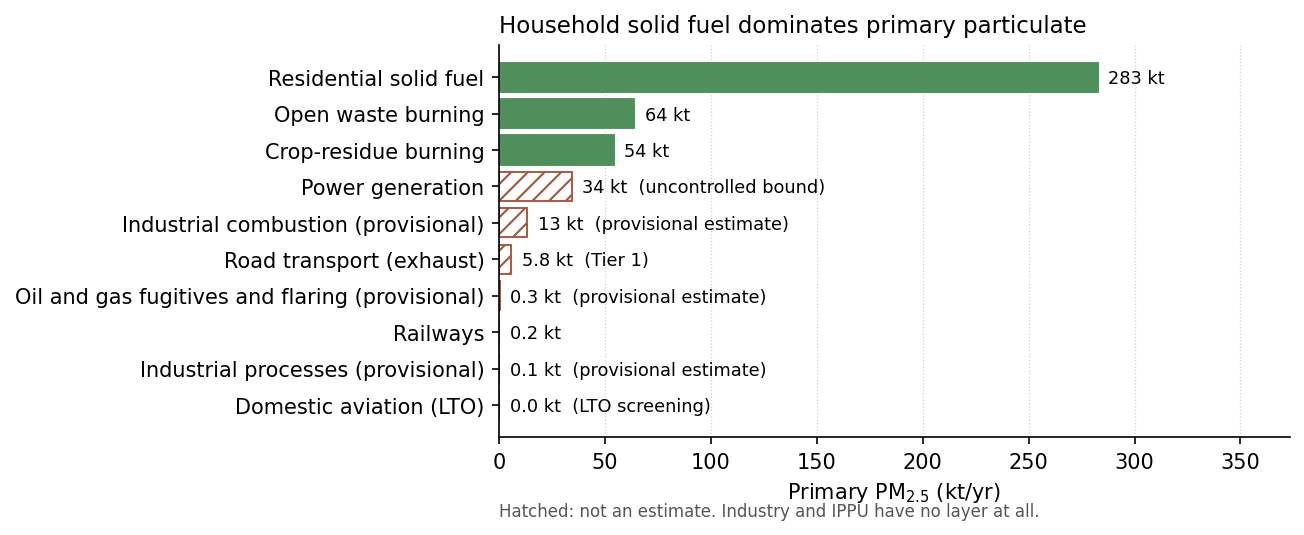
\includegraphics[width=0.86\linewidth]{national_pm25.png}
\caption{Primary \PM{} by combustion source, for the sectors carrying an air-pollutant layer.
Residential solid fuel emits roughly \num{34} times road transport's primary \PM{} under
\texttt{REF\_2023\_24} and \num{77} times under configuration~L, while contributing less than half again its
\COe{}. Hatched bars are the bound and the screening estimate and should not be ranked against
an estimate. Each layer is computed from the same activity quantities as its sector's
greenhouse-gas estimate, so the ordering is a property of combustion conditions rather than of
separate studies with different activity bases.}
\label{fig:pm25}
\end{figure}

\subsection{What the comparison does and does not support}

The policy reading is that the two inventories rank sources almost inversely. A mitigation
programme selected on \COe{} would target transport and electricity; a programme selected on
primary \PM{} emitted would target household cooking and heating first by a wide margin,
followed by two open-burning categories that are together \SI{1.0}{\percent} of the national
inventory. Because each estimate derives from its own sector's activity quantities rather than
from a separate study, that divergence is a real feature of how these fuels burn rather than
an artefact of mismatched activity bases---which is the usual reason such comparisons are
unreliable in developing-country contexts.

Three limits bound how far it can be taken. \emph{Emitted mass is not exposure}: the burden a
population receives depends on where and how each source releases, which this inventory does
not model, so the ordering identifies where the particulate mass originates and not where the
harm lands. \emph{The layer is partial}: the power figures are uncontrolled bounds rather than
what the fleet emits, industrial combustion is a provisional estimate whose equipment shares
are declared rather than surveyed, IPPU process pollutants and fugitive NMVOC are provisional
estimates with urea finishing, nitric acid, lime, glass, venting and post-meter losses typed
absent, and transport omits cold-start, evaporative and non-exhaust processes. And \emph{the assurance
is uneven}, per Table~\ref{tab:airbeta}, which is why this note is labelled beta and why the
main paper reports the one-activity-basis finding without the ranking.

\section{Key categories}
\label{sup:keycat}

The key-category analysis---level against variance, the two rankings it produces and what
the ten-sector trend window can and cannot say---is reported in full in the main article's
Technical validation section (Section~\ref{sec:keycat}) and is not repeated here: a
fragment is printed in one document only, so that the number tests hold each printed value
in exactly one place. This slot is retained so that the supplement's numbering follows the
outline of the data-description article.

% S3: the fragment's own heading is the supplement section.
% ===========================================================================
\section{The Parallel-Table Trap in the IPCC Defaults}
\label{sec:factors}
% ===========================================================================

The 2006 Guidelines \citep{ipcc2006} publish stationary and mobile combustion factors not as
one table per fuel but as several parallel tables, one per source category. Volume~2
Chapter~2 gives four for stationary combustion---energy industries, manufacturing,
commercial, and residential---and Chapter~3 gives separate tables for road, rail and off-road
mobile sources. The same fuel appears in all of them.

Across those tables the \COtwo{} factor for a given fuel is \emph{identical}, because \COtwo{}
depends only on the carbon in the fuel and on complete oxidation. The \CHfour{} and \NtwoO{}
factors are not identical, and in some cases differ by nearly an order of magnitude, because
they depend on how completely and at what temperature the fuel burns.

This creates a failure mode with an unusually bad signature. A compiler who selects the wrong
table gets \COtwo{} exactly right---and \COtwo{} is typically \SIrange{95}{99}{\percent} of a
fossil combustion category, so every obvious check passes. The total looks correct. The
comparison against an external \COtwo{} dataset agrees. Only the trace gases are wrong, and
they can be wrong by a factor large enough to move the affected category by
\SI{8}{\percent}---which is smaller than most published uncertainty bands and therefore
invisible to any validation that works at the level of the total.

\textbf{How much of the total moves depends on how \COtwo{}-dominated the category is, and an
earlier edition of this paper overstated it.} The railway and mixed off-road cases swap
\NtwoO{} between \SI{28.6}{} and \SI{3.9}{\kilo\gram\per\tera\joule} and move their own
category by \SI{8.0}{\percent}. The power and residential cases swap \CHfour{} on gas streams
whose totals are almost entirely \COtwo{}, and move the sector by \SI{0.08}{} and
\SI{0.12}{\percent} respectively---the \CHfour{} row moves several-fold, the total barely at
all. This paper previously reported all four as \SIrange{8}{9}{\percent} sector errors. The
magnitudes are now computed from the engine's activity and the two published factors by
\texttt{tests/test\_factor\_table\_trap.py}, so the claim cannot be restated without the
arithmetic agreeing.

The finding is unharmed by the correction, and is arguably sharper for it. What makes these
errors dangerous is not how much of a total they move but that they move NONE of the
\COtwo{}: every external comparator this inventory has is \COtwo{}-dominated, so all four are
invisible to all of them regardless of size.

We encountered this trap four times in ten sectors. Table~\ref{tab:factortrap} gives all
four instances with the quantified consequence of the plausible error. Each is pinned by a
test that fails if the wrong table's value is ever substituted, and each sector's module
carries the warning in its own documentation with a pointer to its mirror image.

\begin{table*}[htbp]
\centering
\small
\begin{tabular}{@{}p{0.15\linewidth}p{0.13\linewidth}p{0.13\linewidth}p{0.22\linewidth}p{0.27\linewidth}@{}}
\toprule
\textbf{Sector} & \textbf{Correct table} & \textbf{Plausible error} & \textbf{Factor
difference} & \textbf{Consequence of the error} \\
\midrule
Electricity generation (1A1a) &
Vol~2 Ch~2 Table~2.2, Energy Industries &
Table~2.5, Residential &
Natural gas \CHfour{} \SI{1}{\kilo\gram\per\tera\joule} vs \num{5} &
\COtwo{} unchanged; \CHfour{} inflated fivefold. A utility boiler burns far more completely
than a domestic appliance \\[3pt]

Residential fuel (1A4b) &
Vol~2 Ch~2 Table~2.5, Residential &
Table~2.2, Energy Industries &
Natural gas \CHfour{} \SI{5}{\kilo\gram\per\tera\joule} vs \num{1}; kerosene \num{10} vs
\num{3} &
The mirror image: \CHfour{} understated by \SI{80}{\percent} on a quarter of household
energy input \\[3pt]

Railways (1A3c) &
Vol~2 Ch~3 Table~3.4.1, Railways &
Table~3.2.2, Road diesel &
\NtwoO{} \SI{28.6}{\kilo\gram\per\tera\joule} vs \num{3.9}---\num{7.3} times higher &
Railway \NtwoO{} understated by \SI{86}{\percent} and the sector total by about
\SI{9}{\percent}. Large slow-speed locomotive engines run lean at high load, the
\NtwoO{}-forming regime \\[3pt]

Off-road machinery (1A4c) &
Vol~2 Ch~3 Table~3.3.1, Off-road &
Table~3.2.2, Road diesel &
\NtwoO{} \SI{28.6}{\kilo\gram\per\tera\joule} vs \num{3.9} &
The category would report about \SI{8}{\percent} less. Identical to the rail value because
both derive from EEA~2005 and neither engine class generally carries a catalyst \\
\bottomrule
\end{tabular}
\caption{Four instances of the parallel-table trap in this inventory. In every case the
plausible wrong table leaves \COtwo{} exactly correct---so the sector's dominant gas, its
external benchmark comparison and its mass balance all still agree---while the trace gases
move. How far the total moves depends on how \COtwo{}-dominated it is: the railway and
off-road swaps move their own \emph{category} by \SI{8.0}{\percent}, the power and residential
swaps move the \CHfour{} row several-fold and the \emph{sector total} by \SI{0.06}{} and
\SI{0.12}{\percent}. Each magnitude is computed from the engine by a regression test rather
than quoted.}
\label{tab:factortrap}
\end{table*}

\subsection{Why this is a compiler-facing finding rather than a coding note}

Three properties make this worth reporting rather than fixing quietly.

It is \emph{systematic}: it arose in four of the six fuel-burning sectors, and in each case
the wrong table was the one a reasonable person would reach for. The power sector's fuel is
delivered to buildings; the residential sector's largest fossil fuel is natural gas, whose
most familiar factor is the utility one; rail and off-road both burn ordinary road diesel
bought from the same national supply.

It is \emph{invisible to validation}. We compare each sector against EDGAR, FAOSTAT, Climate
TRACE and, where available, Pakistan's own BUR-1. Every one of those comparators is dominated
by \COtwo{} for fossil categories. A sector using the wrong trace-gas table passes all of
them. The only thing that catches it is reading the guidelines carefully enough to notice
that there is more than one table, which is precisely the step under time pressure.

It is \emph{directional}. The errors do not average out. Three of the four instances would
understate the trace gases, because the road and energy-industry tables carry the lower
\CHfour{} and \NtwoO{} values and are the more familiar tables. An inventory community making
this error at random rates would be biased low on non-\COtwo{} combustion emissions.

Two related decisions in the same family are worth recording because they run the other way.
First, we apply \emph{no separate oxidation factor} anywhere in fossil combustion: the 2006
Guidelines assume complete oxidation and fold it into the emission factor, with Table~1.4
carrying an explicit oxidation column of \num{1.0} for every fuel, so applying the
1996-vintage \num{0.98} on top would double-discount. Second, and deliberately contrasting,
the waste sector \emph{does} carry an oxidation factor of \num{0.71}, because open burning
genuinely is incomplete. Both are pinned by tests, so that neither can be ``corrected'' into
the other.

Finally, the power sector's activity is handled on an energy basis rather than a mass basis
for a reason from the same family. IPCC's bituminous and lignite \COtwo{} factors differ by
only \SI{6.8}{\percent} per terajoule but by a factor of two per tonne of coal, because their
net calorific values differ by \SI{54}{\percent} and lignite's own published range spans
\SIrange{5.50}{21.6}{\tera\joule\per\giga\gram}. Working in energy units makes that
uncertainty disappear rather than requiring an assumption about which coal Pakistan burns.


\section{Reproduction, months, geography and sources}
\label{sup:reproduction}

\pkinvDemoteFragment
% ===========================================================================
\section{Reproduction}
\label{app:repro}
% ===========================================================================

The work is split across two repositories along the line this paper draws. This one holds the
inventory: the \texttt{pkinv} Python package, the activity data it reads, the generated
outputs---including the national \SI{0.05}{\degree} monthly cube and its ADM2 view
(Section~\ref{sec:cube})---the tests, this manuscript and the nine sector technical
reports, together with the government source documents that could be retained:
\texttt{data/source\_documents.csv} classifies every activity file as archived, derived
or not-archived, and \num{12} of \num{217} cite at least one document this project used
and does not hold (the provenance audit in Section~\ref{sec:results}). The companion repository holds agriculture
\emph{research} built on top of it---the satellite nowcasting system that estimates emissions
between census years \citep{ahmad2026nowcast}, the machine-learned activity weights and the
agricultural inventory manuscript
\citep{ahmad2026ag}---as the \texttt{pkag} package, which depends on this one. The gridded
surfaces this release distributes are built and tested here, not there.

The agriculture \emph{sector} is computed here rather than there, because it is
\SI{50}{\percent} of the national total and because the residential sector's dung-cake
closure (Section~\ref{sec:closure-dung}) reads its nitrogen flow directly. There is
deliberately no second copy of the activity data in the companion repository: two copies
would drift, which is the failure the closures in Section~\ref{sec:closures} exist to
prevent.

Reproducing the inventory requires Python 3.11 and no compiled dependencies for the core
computation. Every sector exposes a runner:

\begin{verbatim}
python3 -m pkinv.sectors.<sector>.run_<sector>
\end{verbatim}

for nine of the ten sectors; agriculture's runner is
\texttt{python3 -m pkinv.sectors.agriculture.run\_inventory}, the name it carried before the
sector joined the common build. The cross-sector layer is:

\begin{verbatim}
python3 -m pkinv.report.national_rollup
python3 -m pkinv.report.uncertainty_all
python3 -m pkinv.report.key_categories_all
python3 -m pkinv.report.completeness
python3 -m pkinv.report.figures
\end{verbatim}

The full test suite---\num{3882} defined test functions including the \num{32} contract invariants,
the provenance checks, the manuscript number checks and the figure-currency checks---runs
with:

\begin{verbatim}
python3 -m unittest discover tests
\end{verbatim}

All manuscripts compile with \texttt{make papers}, which uses \texttt{tectonic}. Continuous
integration, on each pushed commit, installs the locked environment, runs every sector runner
and the cross-sector layer, runs the test suite, and compiles the national manuscript and one
sector report (railways); the other sector reports, the figure regeneration and the
validation package are the release sequence's job, not CI's, and the release records that
sequence in \texttt{outputs/pakemis\_test\_run.json} and the package's own logs.

\textbf{What that does and does not guarantee.} Defined numerical outputs, registered table
cells, figures, schemas, source references and structural invariants are guarded: a commit in
which any of those disagrees with the engine fails the suite, in CI for pushed commits and in
the release gate for every content commit. \emph{Scientific interpretation and
semantic claims are not guaranteed by the same mechanism.} This paper's own history is the
evidence: a gas decomposition stayed stale for three releases inside a declared-debt list that
tracked it without verifying it; comparative language such as ``doubles'' survived after the
ratio it described had changed; and boundary descriptions drifted between documents. Each of
those classes now has a test---the debt list is gone, comparative claims resolve through a
claims registry, and cross-document boundary statements are checked---but the honest statement
is that the guarantee covers what has been registered, and registration is a choice someone
makes.

% ===========================================================================
\section{Where the months come from}
\label{app:monthly}
% ===========================================================================

Table~\ref{tab:temporal} reports the temporal-evidence class of every module's emissions, as
a share of that module's own total. It is read from \texttt{outputs/temporal\_profile.csv},
which the national run writes beside the monthly layer itself. The largest reconstructed
basis is now electricity generation: NEPRA's Detail-of-Generation listings carry plant-month
generation for the reference year, putting grid coal on TE2 and gas on TE3 (the mixed-labelled
combined-cycle group is assigned to gas by the annual control's own arithmetic, and an
inferred fuel is never graded TE2). The four sectors that anchor on OCAC's monthly
customer-class returns---transport, railways, aviation and industrial combustion---carry the
other substantial reconstructed block, and the TE1 share within
them is the single month of each fiscal year whose cumulative column is the month itself.
Residential is wholly TE3: a degree-day model is a profile built from evidence about the
process rather than a record of these months. Cement was TE3 beside it on a borrowed
calendar-2022 production shape, and is now wholly TE2 - all nine fiscal editions of PBS Table 2
are parsed, so each year carries its own monthly output. It stops short of TE1 because cement
OUTPUT is not clinker CALCINATION, however closely the two track.

\begin{table}[htbp]
\centering
\small
\caption{Temporal evidence by module, as a percentage of each module's own emissions.
TE1 observed monthly, TE2 reconstructed from monthly administrative records, TE3 process-based
profile, TE4 flat and declared. Rows sum to 100 by construction.}
\label{tab:temporal}
\begin{tabular}{@{}lrrrr@{}}
\toprule
\textbf{Module} & \textbf{TE1} & \textbf{TE2} & \textbf{TE3} & \textbf{TE4} \\
\midrule
Agriculture & 0.0 & 7.6 & 8.0 & 84.4 \\
Electricity generation & 0.8 & 48.9 & 38.2 & 12.2 \\
Road transport & 8.4 & 88.5 & 0.0 & 3.1 \\
Residential fuel & 0.0 & 0.0 & 100.0 & 0.0 \\
Industrial combustion & 1.3 & 13.7 & 72.7 & 12.3 \\
Cement (IPPU) & 0.0 & 87.0 & 0.0 & 13.0 \\
Waste & 0.0 & 0.0 & 24.5 & 75.5 \\
Fugitive oil and gas & 0.0 & 43.0 & 0.0 & 57.0 \\
Railways & 6.9 & 93.1 & 0.0 & 0.0 \\
Domestic aviation & 8.0 & 92.0 & 0.0 & 0.0 \\
\bottomrule
\end{tabular}
\end{table}

% ===========================================================================
\section{Where the geography comes from}
\label{app:spatial}
% ===========================================================================

Table~\ref{tab:spatial} is the spatial counterpart of Table~\ref{tab:temporal}: the
spatial-evidence class of every module's emissions, as a share of that module's own total,
read from \texttt{outputs/spatial\_profile.csv}. \textbf{The class is now derived rather than
declared}, and that is this release's second spatial change. It was a literal on each sector
engine, checked against nothing at the point it was written; it is now read from two measured
facts---what the cube's own weight distributes mass by inside each geometry
(\texttt{within\_province\_placement}, one row per geometry set, held against the cube's
dispatch by test) and how many of that set's members that can emit carry a coordinate. Every
stream in this inventory is controlled provincially, because that is the level the activity
statistics exist at, so the class is not about what binds the total; it is about how mass is
placed \emph{below} the province, which is the only part an allocation invents. The ledger
publishes the declared letter and the derived one side by side and the build fails where they
disagree.

Deriving it moved five sets of streams, in both directions. S1 is native source geometry
consuming observed per-object activity, and domestic aviation is the only module that earns
it: thirty-six of thirty-seven airports located, weighted by PCAA movements per airport. It
was S2 on the reasoning that the LTO cycle's stages are unresolved---a within-airport question
this vocabulary does not ask. S2 is geometry the allocation opens without observed per-object
activity at full coverage: railways, whose track is native geometry but whose corridor
service tiers are declared judgement; captive power, where \num{1068} of \num{1105}
registered plants are geocoded and \num{864} carry a gas allocation to weight them by;
and, since this release, the grid fleet at its own plant-ledger fuel and the cement
works at their company's census clinker---partial-coverage point allocations whose
fallbacks are declared ledger events. S3, \SI{71.79}{\percent} of the inventory, is an
administrative statistic: provincial fuel sales, registrations, census counts, downscaled on
declared proxies. The remaining \SI{0.05}{\percent} is NA---not a weaker placement but no
sub-provincial placement at all.

A third axis, and the one a reader is most likely to need and least likely to ask for: whether
the place a stream is put is where it is \emph{emitted}. \SI{82.09}{\percent} of the inventory
is \texttt{physical}. \SI{8.42}{\percent} is \texttt{origin} --- the waste streams, placed at
the people who generate the waste, while the methane leaves landfills, drains and burn sites
for which no allocation-grade geometry is held. \SI{9.50}{\percent} is \texttt{accounting}
--- road, off-road and industrial fuel, booked by OCAC and OGRA to the province of \emph{sale}
and burnt wherever the vehicle or the boiler is. So \SI{79.71}{\mega\tonne},
\SI{17.91}{\percent} of the national total, is placed somewhere other than where it is
emitted, and until this release every product added the three together and returned one
number. \texttt{pakemis\_adm2\_monthly.csv} now carries the view as a dimension, so no row
mixes them and summing across them is a deliberate act; \texttt{spatial\_view\_profile.csv}
publishes the split. This axis is declared rather than derived, because it is a property of
what an activity statistic means and no register holds that; what is enforced instead is that
a stream which is not physical must name the release geography it does not have.

The largest class move when the derivation landed was the grid power fleet from S2 to S3
---a located fleet the allocation ignored was not a facility proxy---and the largest move
since is the same fleet back to S2, EARNED this time: the cube now routes each grid fuel
stream through its corroborated stations at their own plant-ledger fuel, with the
built-up fallback a declared event per province, and the cement register follows at its
company-grained census clinker. The two LNG terminals stay unlocated as a typed refusal:
no held source corroborates a coordinate, and a berth anyone can find on a map is still
a coordinate this register cannot defend.

The classes describe \emph{allocation evidence}, not coverage. A second, orthogonal axis
records whether any geometry
exists at all: \num{3} cruise-aviation streams (\SI{0.06}{\percent} of the national total)
carry the geometry class \texttt{S4:no-native-geometry}, meaning a provincial activity
control with nothing beneath it. They are \emph{not} in the gridded cube. Industry carried
this class through one release candidate - a provincial control and a promise - until rc47
placed it on its own registers (kiln points, the clinker register, built-up); what remains
is fuel burned en route, published in \texttt{pakemis\_spatial\_unallocated.csv}. The
grid total is therefore strictly less than the national total, by exactly that
\SI{0.05}{\percent}, and the identity a reader reconstructs is
\texttt{ADM1 == ADM2 + unallocated} rather than \texttt{ADM1 == ADM2}.

\begin{table}[htbp]
\centering
\small
\caption{Spatial evidence by module, as a percentage of each module's own emissions.
S1 native source geometry, S2 facility or network proxy, S3 administrative statistic on a
declared downscaling proxy. \textbf{NA is not a fourth quality of placement---it is the absence
of one.} The S1--S3 scale grades how mass is placed \emph{below the province}, so a stream that
is controlled at ADM1 and retained whole rather than spread has nothing on that scale to be.
Industrial combustion read \SI{100}{\percent} S3 until this release, asserting an
administrative allocation beneath the province that does not exist; its
\num{30} streams briefly read NA before rc47 Wave 4 placed them on their own
registers; the NA set is now the \num{3} cruise-aviation streams in
\texttt{pakemis\_spatial\_unallocated.csv}. Those streams still carry a province---what they
lack is a level beneath it---and the decomposition's \texttt{placement\_status} and
\texttt{finest\_placement\_level} columns say so, which keeps evidence quality and product
availability in separate fields. Rows sum to 100 by construction.}
\label{tab:spatial}
\begin{tabular}{@{}lrrrr@{}}
\toprule
\textbf{Module} & \textbf{S1} & \textbf{S2} & \textbf{S3} & \textbf{NA} \\
\midrule
Agriculture & 0.0 & 0.0 & 100.0 & 0.0 \\
Electricity generation & 87.78 & 12.22 & 0.0 & 0.0 \\
Road transport & 0.0 & 0.0 & 100.0 & 0.0 \\
Residential fuel & 0.0 & 0.0 & 100.0 & 0.0 \\
Industrial combustion & 0.0 & 60.1 & 39.9 & 0.0 \\
Cement (IPPU) & 0.0 & 85.4 & 14.6 & 0.0 \\
Waste & 0.0 & 89.8 & 10.2 & 0.0 \\
Fugitive oil and gas & 43.0 & 0.5 & 56.5 & 0.0 \\
Railways & 0.0 & 100.0 & 0.0 & 0.0 \\
Domestic aviation & 16.5 & 0.0 & 0.0 & 83.5 \\
\midrule
\textbf{National} & \textbf{11.27} & \textbf{16.88} & \textbf{71.79} & \textbf{0.06} \\
\bottomrule
\end{tabular}
\end{table}

% ===========================================================================
\section{Sources}
\label{app:sources}
% ===========================================================================

Activity data are drawn from Pakistani national and provincial statistics: the Pakistan
Statistical Year Book and the 2023 Population and Housing Census \citep{pbscensus2023} from
the Pakistan Bureau of Statistics; NEPRA's State of Industry Report for electricity fuel
consumption; OGRA's petroleum statistics for road, residential and aviation fuel; Pakistan
Railways Year Books for rail traction fuel; the Punjab Statistical Bureau's provincial
statistics for cement production; the Economic Survey of Pakistan \citep{econsurvey2024ag} and the
Ministry of National Food Security and Research \citep{mnfsrcrops} for agricultural activity;
and the National Fertilizer Development Centre \citep{nfdc2024} for fertiliser. The two
agricultural citations name the FY2023--24 editions this release reads and archives, not the
FY2024--25 editions published since \citep{econsurvey,nfdc2025}.
International sources are used where no national equivalent exists and are flagged as
such in the provenance table. FAOSTAT \citep{faostat} is \emph{not} among the principal ones
any more: household firewood is now the HIES survey's own measured consumption, and FAOSTAT
survives as a structural comparison against it rather than as the activity basis.

Emission factors are IPCC 2006 Guidelines defaults \citep{ipcc2006} with the 2019 Refinement
\citep{ipcc2019} applied where it supersedes them, except in the agriculture sector's Tier~2
elements \citep{ahmad2026ag}. Every factor in the repository cites its source table, and a
test asserts that no factor lacks a citation and that any informally sourced value is
explicitly declared as such.

\pkinvEndFragment

% S5: generated/claim_matrix.tex is written by scripts/make_claim_matrix.py and carries
% its own heading.
% GENERATED by scripts/make_claim_matrix.py from data/claim_matrix.csv - do not edit.
\subsection*{S5 The claim matrix}
\label{sec:claim-matrix}

Every headline claim of the national paper is a row of \texttt{data/claim\_matrix.csv}: the sentence as printed, its quantity references into the claims machinery, the source pointer, the stored query, the configuration, unit and rounding, the evidence class, the limitation paragraph it is bounded by, the technical notes it rests on and the artefact that shows it. \texttt{scripts/make\_claim\_matrix.py} resolves each row against the release and writes \texttt{outputs/pakemis\_claim\_matrix.csv}; the tables below print the identifier, the printed and resolved values, the evidence class and the limitation label. The sentence itself, the pointer and the query parameters are in the CSV. A row whose printed value disagrees with the release fails \texttt{tests/paper\_numbers/test\_claim\_matrix.py}; nothing is repaired in place.

\begin{table}[htbp]
\centering
\footnotesize
\setlength{\tabcolsep}{4pt}
\caption{Claim matrix: Abstract.}
\begin{tabular}{@{}p{3.6cm}lrrp{2.6cm}p{2.4cm}@{}}
\toprule
\textbf{claim} & \textbf{via} & \textbf{printed} & \textbf{resolved} & \textbf{evidence} & \textbf{limitation} \\
\midrule
abs\_\allowbreak{}total\_\allowbreak{}L & query & 444.96 & 444.96 & closure-exact & incomplete-floor \\
abs\_\allowbreak{}total\_\allowbreak{}AR6 & query & 438.19 & 438.19 & closure-exact &  \\
abs\_\allowbreak{}total\_\allowbreak{}S & query & 450.20 & 450.20 & structural & incomplete-floor \\
abs\_\allowbreak{}flat\_\allowbreak{}share & pointer & 54.65 & 54.65 & estimated-TE4 & monthly-physics \\
abs\_\allowbreak{}streams\_\allowbreak{}gridded & pointer & 199 & 199 & coverage-count &  \\
abs\_\allowbreak{}streams\_\allowbreak{}total & pointer & 202 & 202 & coverage-count &  \\
abs\_\allowbreak{}streams\_\allowbreak{}unallocated & pointer & 3 & 3 & spatial-S4 &  \\
abs\_\allowbreak{}unallocated\_\allowbreak{}share & pointer & 0.05 & 0.06 & spatial-S4 &  \\
abs\_\allowbreak{}mc\_\allowbreak{}interval & pointer & 11.72 & 11.72 & parametric &  \\
abs\_\allowbreak{}mc\_\allowbreak{}down & pointer & 10.3 & 10.3 & parametric &  \\
abs\_\allowbreak{}mc\_\allowbreak{}up & pointer & 13.1 & 13.1 & parametric &  \\
abs\_\allowbreak{}structural\_\allowbreak{}max & pointer & 9.07 & 9.1 & structural &  \\
abs\_\allowbreak{}legacy\_\allowbreak{}control\_\allowbreak{}delta & pointer & 17.78 & 17.8 & structural &  \\
abs\_\allowbreak{}completeness\_\allowbreak{}rows & query & 138 & 138 & coverage-count & incomplete-floor \\
abs\_\allowbreak{}completeness\_\allowbreak{}E & query & 54 & 54 & coverage-count & incomplete-floor \\
abs\_\allowbreak{}completeness\_\allowbreak{}NE & query & 71 & 71 & coverage-count & incomplete-floor \\
\bottomrule
\end{tabular}
\end{table}

\begin{table}[htbp]
\centering
\footnotesize
\setlength{\tabcolsep}{4pt}
\caption{Claim matrix: 1 Introduction.}
\begin{tabular}{@{}p{3.6cm}lrrp{2.6cm}p{2.4cm}@{}}
\toprule
\textbf{claim} & \textbf{via} & \textbf{printed} & \textbf{resolved} & \textbf{evidence} & \textbf{limitation} \\
\midrule
intro\_\allowbreak{}contract\_\allowbreak{}tests & getter & 32 & 32 & provenance-count &  \\
intro\_\allowbreak{}enteric\_\allowbreak{}share & pointer & 34.1 & 34.1 & closure-exact &  \\
intro\_\allowbreak{}residential\_\allowbreak{}share & pointer & 5.4 & 5.4 & closure-exact &  \\
intro\_\allowbreak{}total\_\allowbreak{}L & query & 444.96 & 444.96 & closure-exact & incomplete-floor \\
intro\_\allowbreak{}edgar\_\allowbreak{}magnitude & pointer & 87 & 86 & external-comparison & incomplete-floor \\
intro\_\allowbreak{}edgar\_\allowbreak{}scope & pointer & 11 & 11 & external-comparison & incomplete-floor \\
intro\_\allowbreak{}completeness\_\allowbreak{}rows & query & 138 & 138 & coverage-count &  \\
intro\_\allowbreak{}contract\_\allowbreak{}invariants & getter & 32 & 32 & provenance-count &  \\
intro\_\allowbreak{}residual\_\allowbreak{}variance & pointer & 2.5 & 2.5 & parametric &  \\
\bottomrule
\end{tabular}
\end{table}

\begin{table}[htbp]
\centering
\footnotesize
\setlength{\tabcolsep}{4pt}
\caption{Claim matrix: 2 Dataset scope and architecture.}
\begin{tabular}{@{}p{3.6cm}lrrp{2.6cm}p{2.4cm}@{}}
\toprule
\textbf{claim} & \textbf{via} & \textbf{printed} & \textbf{resolved} & \textbf{evidence} & \textbf{limitation} \\
\midrule
tab\_\allowbreak{}completeness\_\allowbreak{}rows & query & 138 & 138 & coverage-count & incomplete-floor \\
tab\_\allowbreak{}completeness\_\allowbreak{}codes & pointer & 72 & 72 & coverage-count & incomplete-floor \\
\bottomrule
\end{tabular}
\end{table}

\begin{table}[htbp]
\centering
\footnotesize
\setlength{\tabcolsep}{4pt}
\caption{Claim matrix: 4 Dataset generation.}
\begin{tabular}{@{}p{3.6cm}lrrp{2.6cm}p{2.4cm}@{}}
\toprule
\textbf{claim} & \textbf{via} & \textbf{printed} & \textbf{resolved} & \textbf{evidence} & \textbf{limitation} \\
\midrule
tab\_\allowbreak{}sectors\_\allowbreak{}total & query & 444.96 & 444.96 & closure-exact &  \\
fig\_\allowbreak{}sectors\_\allowbreak{}agriculture\_\allowbreak{}share & pointer & 50.2 & 50.2 & closure-exact &  \\
tab\_\allowbreak{}categorygas\_\allowbreak{}CH4 & query & 242.932 & 242.932 & closure-exact &  \\
tab\_\allowbreak{}categorygas\_\allowbreak{}CO2 & query & 160.944 & 160.944 & closure-exact &  \\
tab\_\allowbreak{}categorygas\_\allowbreak{}N2O & query & 41.079 & 41.079 & closure-exact &  \\
fig\_\allowbreak{}series\_\allowbreak{}first\_\allowbreak{}year & query & 393.84 & 393.84 & closure-exact & series-basis \\
fig\_\allowbreak{}series\_\allowbreak{}window\_\allowbreak{}change & query & 51.12 & 51.12 & closure-exact & series-basis \\
fig\_\allowbreak{}seasonality\_\allowbreak{}closure & query & 444.96 & 444.96 & closure-exact &  \\
fig\_\allowbreak{}seasonality\_\allowbreak{}flat\_\allowbreak{}share & pointer & 54.65 & 54.65 & estimated-TE4 & monthly-physics \\
tab\_\allowbreak{}correlation\_\allowbreak{}national & pointer & 11.72 & 11.72 & parametric &  \\
tab\_\allowbreak{}correlation\_\allowbreak{}national\_\allowbreak{}correlated & pointer & 11.75 & 11.75 & parametric &  \\
fig\_\allowbreak{}bridge\_\allowbreak{}largest & pointer & 9.1 & 9.1 & structural &  \\
tab\_\allowbreak{}dungvariants\_\allowbreak{}difference & query & 5.2 & 5.2 & structural & incomplete-floor \\
res\_\allowbreak{}streams\_\allowbreak{}gridded & pointer & 199 & 199 & coverage-count &  \\
res\_\allowbreak{}streams\_\allowbreak{}unallocated & pointer & 3 & 3 & spatial-S4 &  \\
res\_\allowbreak{}agri\_\allowbreak{}misaligned\_\allowbreak{}crops & pointer & 3 & 3 & coverage-count & series-basis \\
res\_\allowbreak{}agri\_\allowbreak{}calendar\_\allowbreak{}share & pointer & 77.37 & 77.37 & estimated-TE4 & series-basis \\
res\_\allowbreak{}agri\_\allowbreak{}basis\_\allowbreak{}change & pointer & -7.6969 & -7.6969 & structural & series-basis \\
res\_\allowbreak{}agri\_\allowbreak{}cotton\_\allowbreak{}scope & pointer & 1.055 & 1.055 & structural & series-basis \\
unc\_\allowbreak{}trend\_\allowbreak{}changes\_\allowbreak{}tested & pointer & 8 & 8 & parametric & series-basis \\
unc\_\allowbreak{}trend\_\allowbreak{}changes\_\allowbreak{}resolved & pointer & 2 & 2 & parametric & series-basis \\
unc\_\allowbreak{}trend\_\allowbreak{}common\_\allowbreak{}window & pointer & 51.12 & 51.12 & parametric & series-basis \\
unc\_\allowbreak{}variance\_\allowbreak{}persists & pointer & 76.56 & 76.56 & parametric &  \\
unc\_\allowbreak{}variance\_\allowbreak{}residual & pointer & 2.48 & 2.48 & parametric &  \\
spatial\_\allowbreak{}adm1\_\allowbreak{}by\_\allowbreak{}year\_\allowbreak{}rows & pointer & 7864 & 7864 & coverage-count &  \\
spatial\_\allowbreak{}adm2\_\allowbreak{}by\_\allowbreak{}year\_\allowbreak{}rows & pointer & 10350 & 10350 & coverage-count &  \\
spatial\_\allowbreak{}grid\_\allowbreak{}fleet\_\allowbreak{}substituted\_\allowbreak{}fy2015\_\allowbreak{}16 & getter & 17.66 & 17.66 & spatial-S4 &  \\
spatial\_\allowbreak{}stream\_\allowbreak{}years\_\allowbreak{}own\_\allowbreak{}year & getter & 795 & 795 & provenance-count &  \\
spatial\_\allowbreak{}stream\_\allowbreak{}years\_\allowbreak{}backcast & pointer & 306 & 306 & provenance-count &  \\
spatial\_\allowbreak{}adm2\_\allowbreak{}monthly\_\allowbreak{}by\_\allowbreak{}year\_\allowbreak{}rows & pointer & 122616 & 122616 & coverage-count &  \\
spatial\_\allowbreak{}stream\_\allowbreak{}years\_\allowbreak{}timeless & pointer & 615 & 615 & provenance-count &  \\
\bottomrule
\end{tabular}
\end{table}

\begin{table}[htbp]
\centering
\footnotesize
\setlength{\tabcolsep}{4pt}
\caption{Claim matrix: 6 Technical validation.}
\begin{tabular}{@{}p{3.6cm}lrrp{2.6cm}p{2.4cm}@{}}
\toprule
\textbf{claim} & \textbf{via} & \textbf{printed} & \textbf{resolved} & \textbf{evidence} & \textbf{limitation} \\
\midrule
tab\_\allowbreak{}benchmarks\_\allowbreak{}magnitude & pointer & 87 & 86 & external-comparison & incomplete-floor \\
\bottomrule
\end{tabular}
\end{table}

\begin{table}[htbp]
\centering
\footnotesize
\setlength{\tabcolsep}{4pt}
\caption{Claim matrix: 7 Usage notes and limitations.}
\begin{tabular}{@{}p{3.6cm}lrrp{2.6cm}p{2.4cm}@{}}
\toprule
\textbf{claim} & \textbf{via} & \textbf{printed} & \textbf{resolved} & \textbf{evidence} & \textbf{limitation} \\
\midrule
lim\_\allowbreak{}single\_\allowbreak{}year\_\allowbreak{}period & pointer & FY2023--24 & FY2023-24 & coverage-count & single-year \\
lim\_\allowbreak{}floor\_\allowbreak{}edgar\_\allowbreak{}1a2 & pointer & 44 & 44 & external-comparison & incomplete-floor \\
lim\_\allowbreak{}floor\_\allowbreak{}industry\_\allowbreak{}gas & getter & 5.61 & 5.61 & closure-exact & incomplete-floor \\
lim\_\allowbreak{}floor\_\allowbreak{}1a2\_\allowbreak{}remaining & pointer & 15.85 & 16 & external-comparison & incomplete-floor \\
lim\_\allowbreak{}floor\_\allowbreak{}chemical\_\allowbreak{}filing & pointer & 19.4 & 19.4 & external-comparison & incomplete-floor \\
lim\_\allowbreak{}floor\_\allowbreak{}commercial & getter & 2.4 & 2.4 & structural & incomplete-floor \\
lim\_\allowbreak{}floor\_\allowbreak{}total\_\allowbreak{}rounded & query & 445 & 445 & closure-exact & incomplete-floor \\
lim\_\allowbreak{}floor\_\allowbreak{}dung\_\allowbreak{}ratio & getter & 4.9 & 4.9 & structural & incomplete-floor \\
lim\_\allowbreak{}floor\_\allowbreak{}config\_\allowbreak{}difference & query & 5.25 & 5.25 & structural & incomplete-floor \\
lim\_\allowbreak{}lulucf\_\allowbreak{}sink & pointer & -4.01 & -4.01 & structural & lulucf \\
lim\_\allowbreak{}fugitives\_\allowbreak{}floor & pointer & 9.601 & 9.601 & structural & fugitive-envelope \\
lim\_\allowbreak{}fugitives\_\allowbreak{}top & pointer & 23.499 & 23.499 & structural & fugitive-envelope \\
lim\_\allowbreak{}fugitives\_\allowbreak{}lower & pointer & 14.894 & 14.894 & structural & fugitive-envelope \\
lim\_\allowbreak{}series\_\allowbreak{}first\_\allowbreak{}fy & pointer & FY2015--16 & FY2015-16 & coverage-count & series-basis \\
lim\_\allowbreak{}series\_\allowbreak{}calendar\_\allowbreak{}share & pointer & 77.37 & 77.37 & estimated-TE4 & series-basis \\
lim\_\allowbreak{}series\_\allowbreak{}ne\_\allowbreak{}years & pointer & no & 0 & coverage-count & series-basis \\
lim\_\allowbreak{}firewood\_\allowbreak{}energy\_\allowbreak{}share & getter & 38.7 & 38.7 & structural & firewood \\
lim\_\allowbreak{}dung\_\allowbreak{}energy\_\allowbreak{}share & getter & 13.6 & 13.6 & structural & firewood \\
lim\_\allowbreak{}firewood\_\allowbreak{}uncertainty & pointer & 35 & 35 & parametric & firewood \\
lim\_\allowbreak{}firewood\_\allowbreak{}faostat & pointer & 23.89 & 23.89 & structural & firewood \\
lim\_\allowbreak{}firewood\_\allowbreak{}excluded & pointer & 20.81 & 20.81 & structural & firewood \\
lim\_\allowbreak{}monthly\_\allowbreak{}flat\_\allowbreak{}share & pointer & 54.65 & 54.65 & estimated-TE4 & monthly-physics \\
lim\_\allowbreak{}monthly\_\allowbreak{}observed & pointer & 37.3 & 37.3 & estimated-TE2 & monthly-physics \\
lim\_\allowbreak{}monthly\_\allowbreak{}physical & pointer & 41.0 & 41.0 & estimated-TE4 & monthly-physics \\
lim\_\allowbreak{}monthly\_\allowbreak{}weakly\_\allowbreak{}timed & pointer & 21.8 & 21.8 & estimated-TE4 & monthly-physics \\
lim\_\allowbreak{}grade\_\allowbreak{}nine\_\allowbreak{}year & getter & 21.76 & 21.76 & estimated-TE4 & monthly-grade \\
lim\_\allowbreak{}grade\_\allowbreak{}reference\_\allowbreak{}year & getter & 9.57 & 9.57 & estimated-TE4 & monthly-grade \\
lim\_\allowbreak{}grade\_\allowbreak{}target & getter & 15 & 15 & estimated-TE4 & monthly-grade \\
lim\_\allowbreak{}grade\_\allowbreak{}ocac\_\allowbreak{}mass & getter & 283.2 & 283.2 & estimated-TE4 & monthly-grade \\
lim\_\allowbreak{}grade\_\allowbreak{}after\_\allowbreak{}ocac & getter & 14.68 & 14.68 & estimated-TE4 & monthly-grade \\
lim\_\allowbreak{}managed\_\allowbreak{}soils\_\allowbreak{}moved & getter & 95.09 & 95.11 & estimated-TE2 & monthly-gap \\
lim\_\allowbreak{}agriculture\_\allowbreak{}cells & getter & 72 & 72 & closure-exact & monthly-gap \\
\bottomrule
\end{tabular}
\end{table}

\begin{table}[htbp]
\centering
\footnotesize
\setlength{\tabcolsep}{4pt}
\caption{Claim matrix: 7 Usage notes and limitations (continued).}
\begin{tabular}{@{}p{3.6cm}lrrp{2.6cm}p{2.4cm}@{}}
\toprule
\textbf{claim} & \textbf{via} & \textbf{printed} & \textbf{resolved} & \textbf{evidence} & \textbf{limitation} \\
\midrule
lim\_\allowbreak{}fugitives\_\allowbreak{}moved & getter & 93.66 & 93.66 & estimated-TE2 & monthly-gap \\
lim\_\allowbreak{}fugitives\_\allowbreak{}t2\_\allowbreak{}share & getter & 43.0 & 43.0 & estimated-TE2 & monthly-gap \\
lim\_\allowbreak{}deposit\_\allowbreak{}sources & pointer & 217 & 217 & provenance-count & deposit \\
lim\_\allowbreak{}deposit\_\allowbreak{}archived & pointer & 153 & 153 & provenance-count & deposit \\
lim\_\allowbreak{}deposit\_\allowbreak{}no\_\allowbreak{}terms & pointer & 126 & 126 & provenance-count & deposit \\
lim\_\allowbreak{}deposit\_\allowbreak{}sources\_\allowbreak{}restated & pointer & 217 & 217 & provenance-count & deposit \\
lim\_\allowbreak{}deposit\_\allowbreak{}files & pointer & 1761 & 1761 & provenance-count & deposit \\
\bottomrule
\end{tabular}
\end{table}

\begin{table}[htbp]
\centering
\footnotesize
\setlength{\tabcolsep}{4pt}
\caption{Claim matrix: 10 Conclusions.}
\begin{tabular}{@{}p{3.6cm}lrrp{2.6cm}p{2.4cm}@{}}
\toprule
\textbf{claim} & \textbf{via} & \textbf{printed} & \textbf{resolved} & \textbf{evidence} & \textbf{limitation} \\
\midrule
concl\_\allowbreak{}total\_\allowbreak{}L & query & 444.96 & 444.96 & closure-exact & incomplete-floor \\
concl\_\allowbreak{}contract\_\allowbreak{}invariants & getter & 32 & 32 & provenance-count &  \\
concl\_\allowbreak{}factor\_\allowbreak{}trap & getter & 8.0 & 8.0 & structural &  \\
concl\_\allowbreak{}mc\_\allowbreak{}interval & pointer & 11.72 & 11.72 & parametric &  \\
concl\_\allowbreak{}mc\_\allowbreak{}road & pointer & 13.3 & 13.3 & parametric &  \\
concl\_\allowbreak{}wastewater\_\allowbreak{}factor & getter & 1.6 & 1.6 & structural &  \\
concl\_\allowbreak{}edgar\_\allowbreak{}1a2 & pointer & 44 & 44 & external-comparison & incomplete-floor \\
concl\_\allowbreak{}activity\_\allowbreak{}files & pointer & 217 & 217 & provenance-count & deposit \\
\bottomrule
\end{tabular}
\end{table}

$^{\dagger}$ printed value outside the DOC\_CLAIMS agreement rule at the time of rendering.


\bibliographystyle{elsarticle-harv}
\bibliography{../../../paper_common/references}

\end{document}
